À des fins prospectives, on souhaite modéliser le capital d'une entreprise qui fabrique et vend un produit. On utilise les notations suivantes.

\begin{itemize}[label=\small\textbullet]
	\item $C(x)$ est le coût de production en euros pour $x$ unités produites.

	\item $C_m(x) = C(x) - C(x - 1)$ est le coût marginal de production pour $x \in \NNs$ \textit{(c'est le coût spécifique à la x\ieme unité produite)}.
	
	\item $CM(x) = \dfrac{C(x)}{x}$ est le coût moyen de production pour $x \in \NNs$.
\end{itemize}


% ---------------- %


\paragraph{Cas 1.}

Supposons que des études statistiques aient montré que lorsque le nombre d'unités vendues augmente le coût marginal évolue de façon quasi linéaire.

Dans ce cas, on peut faire l'approximation $C_m(x) = ax + b$ avec $(a ; b) \in \left( \RRsp \right)^2$ \emph{(cette fonction affine peut être celle obtenue via une régression linéaire par la méthode des moindres carrés)}. Nous avons alors :
\begin{flalign*}
	C(x) &= C(0) + \sum_{k = 1}^{x} C_m(k) & \\
	     &= C(0) + \sum_{k = 1}^{x} (a k + b) & \\
	     &= m x^2 + p x + q & \\
\end{flalign*}

\vspace{-2em}


Pour la dernière égalité, nous avons utilisé le fait que $\forall (e, x) \in \NN \times \NNs$ , $\displaystyle \sum_{k = 1}^{x} k^e$ est un polynôme en $x$ de degré $(e + 1)$ . En utilisant les formules exactes de ces polynômes, il est facile de vérifier que nos coefficients $m$ , $p$ et $q$ sont tous positifs et même que $m > 0$ .


\bigskip

Avec ce modèle, nous avons $CM(x) = m x + p + \frac{q}{x}$ pour $x \in \NNs$. Nous pouvons donner l'interprétation concrète suivante des termes $mx$ , $p$ et $\frac{q}{x}$ . 

\begin{enumerate}
	\item $p$ correspond à un coût fixe de fabrication : quelque soit le nombre d'unités vendues, l'entreprise doit débourser en moyenne $q$ euros par unité fabriquée 
	\emph{(penser à l'usage de bâtiments, aux salaires des employés en CDI...)}.


	\item $mx$ augmente strictement avec $x$ car $m > 0$. Ce terme correspond à un coût d'usage
	\emph{(penser par exemple à l'entretien d'une chaîne de production, à l'énergie dépensée en plus pour produire plus...)}.


	\item $\frac{q}{x}$ indique un coût amorti en ce sens où plus $x$ augmente moins $\frac{q}{x}$ influence $CM(x)$
	\emph{(penser par exemple à des investissement faits pour une nouvelle chaîne de production)}.
\end{enumerate}


% ---------------- %


\paragraph{Cas 2.}

Supposons que des études statistiques aient montré que lorsque le nombre d'unités vendues augmente le coût marginal diminue strictement puis qu'ensuite il atteint un minimum pour enfin ne cesser d'augmenter strictement.
Notons que le minimum est forcément positif, et la valeur où il est atteint strictement positive.
Nous supposons de plus que les données sont telles que la courbe de $C_m$ soit quasi parabolique.


\medskip


Dans ce cas, on peut faire l'approximation $C_m(x) = ax^2 + bx + c$ avec les contraintes $a > 0$ , $\Delta \stackrel{\text{déf}}{=} b^2 - 4ac \leq 0$ ainsi que $\frac{-b}{2a} > 0$ \emph{(ce polynôme du 2\ieme degré peut être celui obtenu via une régression polynomiale par la méthode des moindres carrés)}. Pourquoi ces conditions ?

\begin{enumerate}
	\item $a > 0$ permet de vérifier les contraintes de variation.


	\item $\Delta \leq 0$ et $\frac{-b}{2a} > 0$ servent à valider la contrainte du minimum.
\end{enumerate}


\medskip


De nouveau, nous avons :
\begin{flalign*}
	C(x) &= C(0) + \sum_{k = 1}^{x} C_m(k) & \\
	     &= C(0) + \sum_{k = 1}^{x} (a k^2 + b k + c) & \\
	     &= m x^3 + p x^2 + q x + r & \\
\end{flalign*}


\vspace{-1em}

\begin{wrapfigure}{r}{0.3\textwidth} 
	\vspace{-.5em}
	\begin{center}
		\fbox{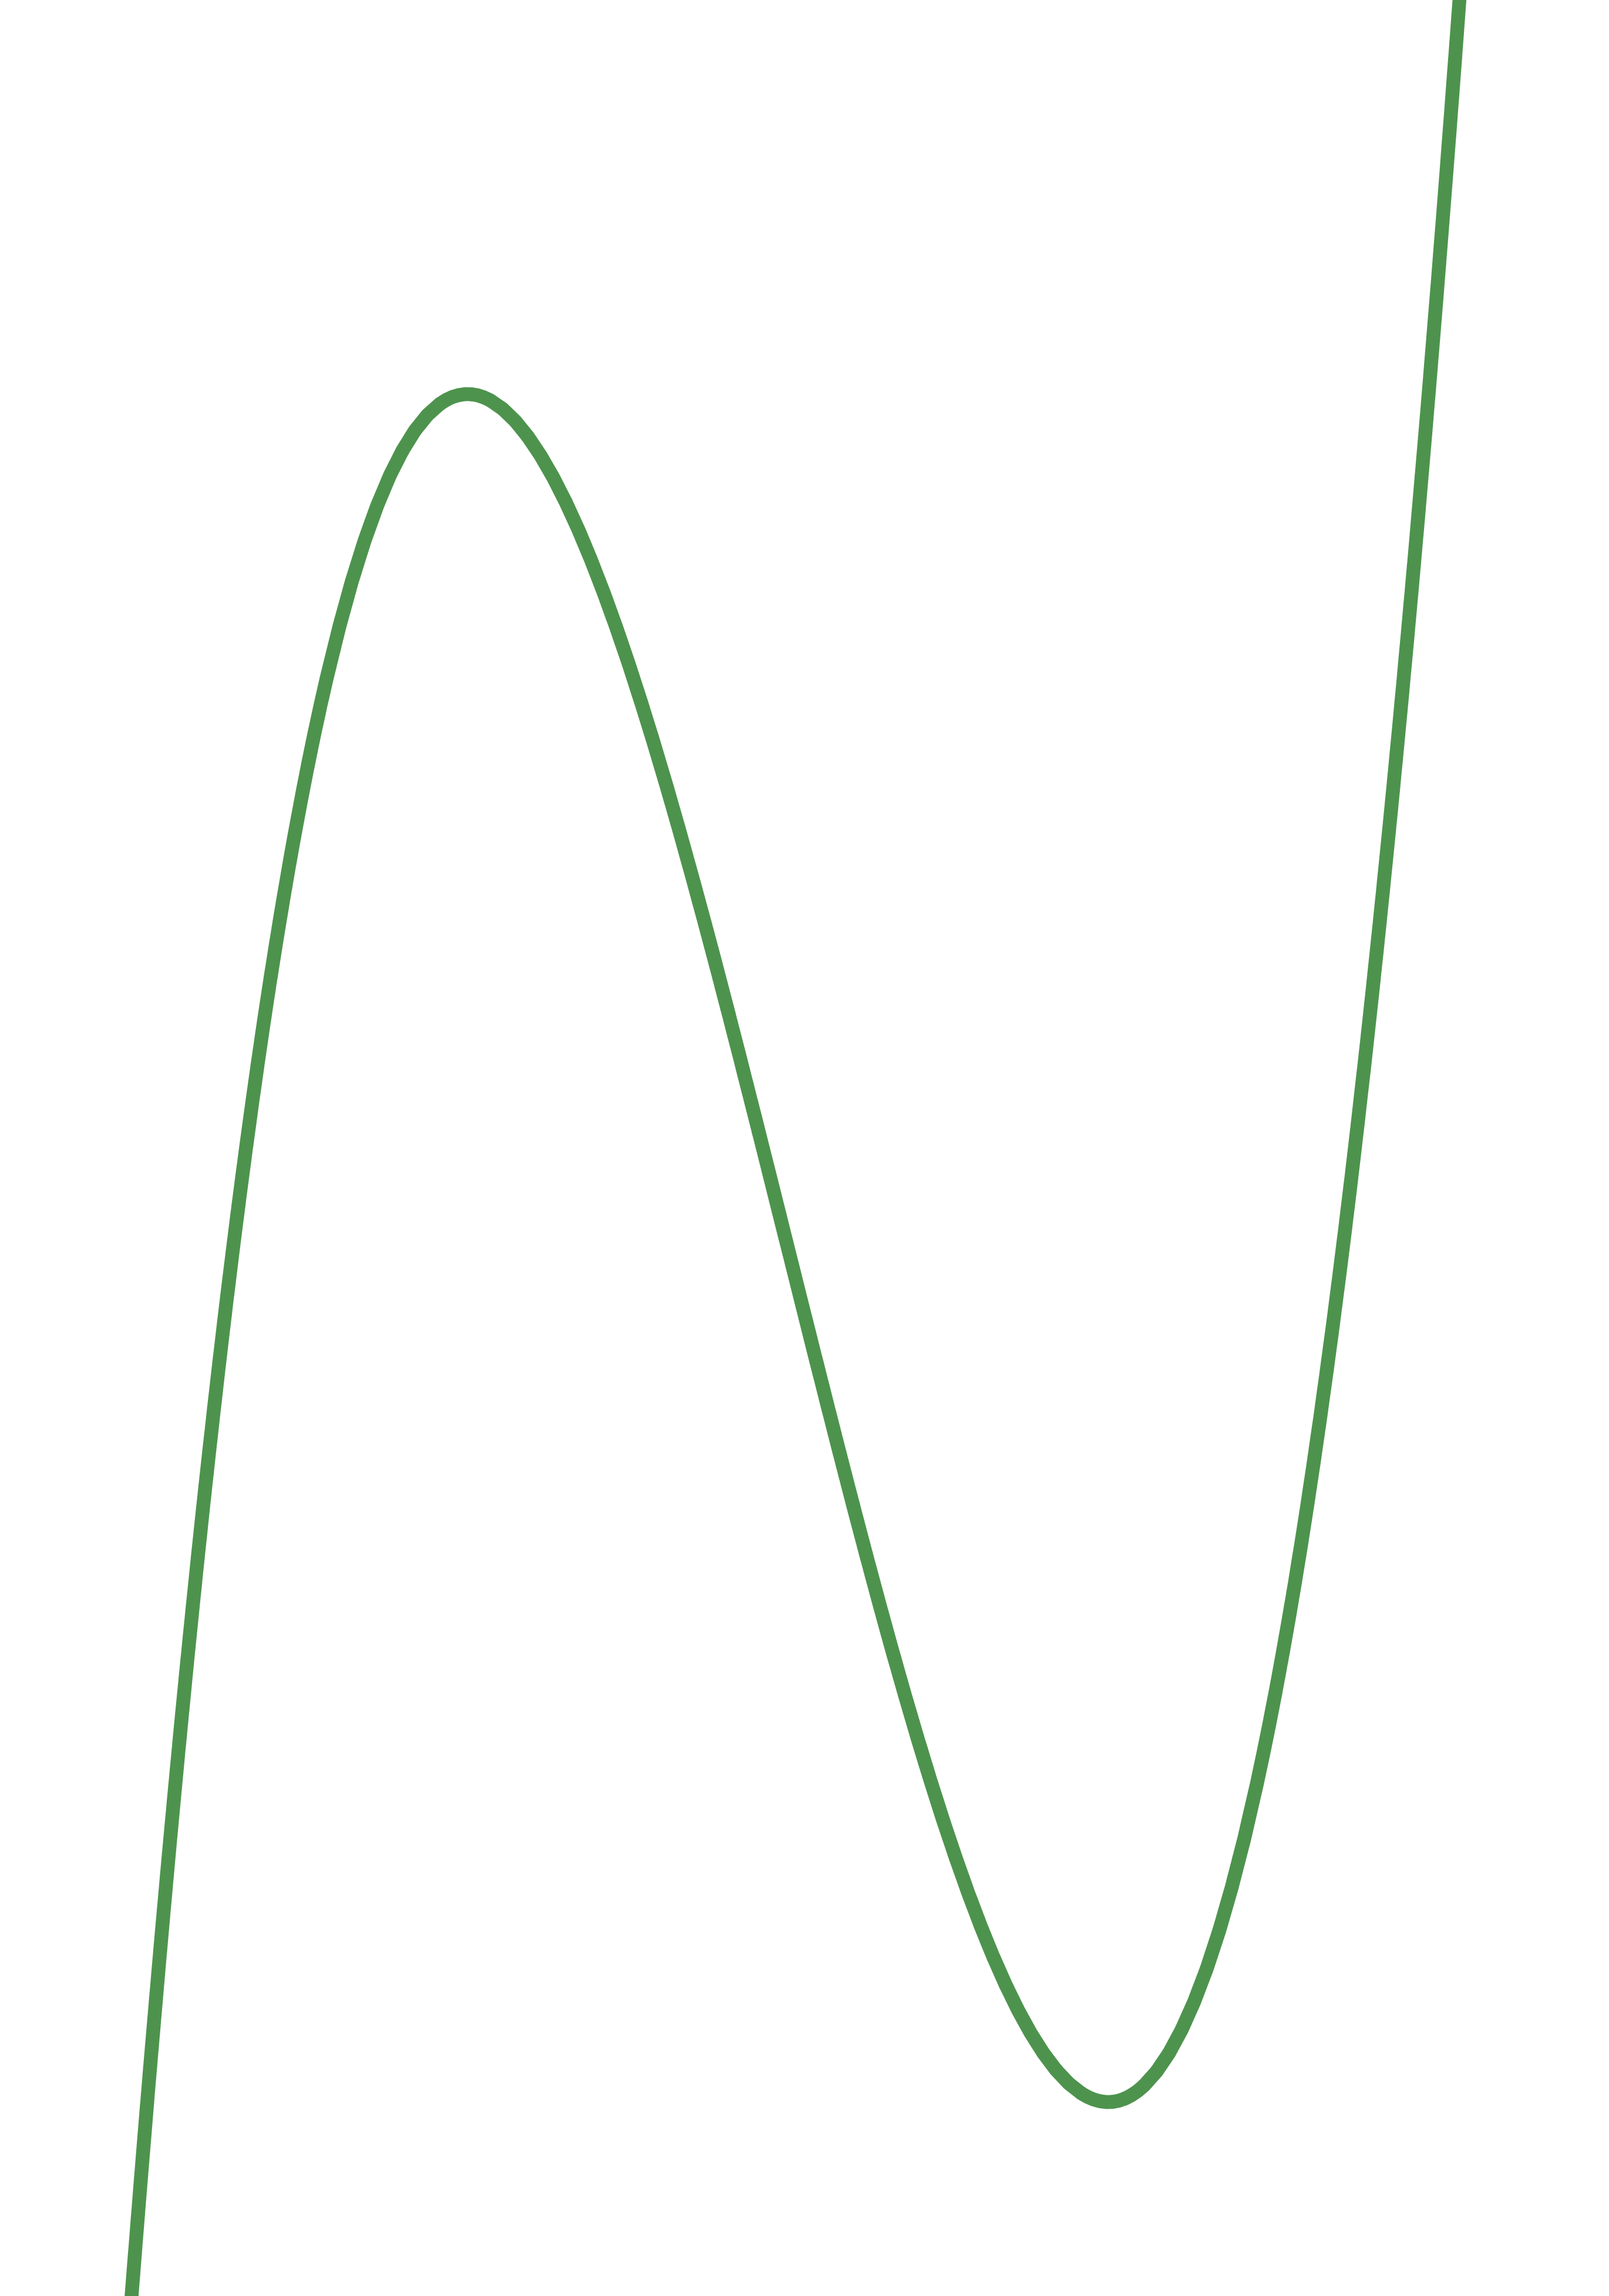
\includegraphics[scale = .4]{cubic.png}}
	\end{center}
	\vspace{-2.25em}
\end{wrapfigure} 

Si une étude statistique rapide sur le coût de fabrication $C$ fournit une courbe similaire à celle ci-contre, on pourra espérer modéliser correctement $C$ avec un polynôme de degré 3 comme ci-dessus. Dans ce cas, il faudra bien choisir  certaines données concrètes afin de trouver de \emph{\og bonnes \fg} valeurs des coefficients $m$ , $p$ , $q$ et $r$ . C'est à l'usage que l'on pourra voir la pertinence ou non de ces choix.


\bigskip

Avec ce modèle, nous avons $CM(x) = m x^2 + p x + q + \frac{r}{x}$ pour $x \in \NNs$.
Bien que les significations concrètes de $p x$ , $q$  et $\frac{r}{x}$ peuvent être similaires à celles données dans le cas 1, il devient difficile de donner un sens concret au terme $m x^2$ .  


% ---------------- %


\begin{remark}
	Si le coût marginal $C_m$ admet une \emph{\og courbe en U \fg}, on pourra faire l'approximation $C_m(x) = c (x - \alpha)^{2p} + \beta$ avec $(c ; \alpha ; \beta) \in \left( \RRp \right)^3$ et $p \in \NNs$ .
	Dans ce cas, $C(x)$ sera un polynôme de degré $(2p + 1)$. Est-ce plus efficace au final que de considérer une \emph{\og courbe en U \fg} comme quasi parabolique ?
	Ne pas oublier qu'un modèle doit être aisément utilisable quitte à être un peu approximatif. Il est donc parfois inutile de vouloir être trop précis.
\end{remark}


% ---------------- %


\begin{remark}
	Plus généralement, on pourrait considérer d'autres types de fonction avec des variations collant à une étude statistique pour peu que le comportement du coût marginal $C_m$ soit relativement régulier. Le problème que l'on aura à résoudre sera soit d'évaluer simplement $\displaystyle \sum_{k = 1}^{x} C_m(k)$ pour une utilisation \emph{\og humaine \fg}, soit de le faire efficacement de façon informatique.
\end{remark}


% ---------------- %


\begin{remark}
	On justifie très souvent les deux modèles précédents via l'utilisation de l'approximation $C_m(x) \approx C\,'(x)$ , puis ensuite on utilise les polynômes ainsi trouvés pour des applications numériques avec de faibles valeurs pour $x$. On voit que cette démarche est fragile
	\footnote{
		L'auteur, qui enseigne les mathématiques au lycée, doit admettre qu'il utilise aussi ce type de raisonnement dans des exercices, ce qui est pédagogiquement intéressant dans le cadre du calcul de dérivées. Par contre, les élèves sont avertis de l'arnaque faite en utilisant l'expression polynomiale pour de petites valeurs de $x$.
	}.
	Le piège est que cette approche fournit tout de même un polynôme de degré $2$ ou $3$ suivant les hypothèses de départ.
	Il pourrait être intéressant d'évaluer l'erreur commise par rapport à la méthodologie présentée dans ce document.
\end{remark}
